\chapter{Literature Review}
\label{chapter:literature-review}

\section{Waterfall Model}
\label{sec:waterfall-model}

The waterfall model is one of the oldest and most well-known software development methodologies and was initially proposed by Winston W. Royce in 1970 \cite{royce70}. The model is characterized by its linear and sequential approach to project management \cite{Novianti2023}. Each phase must be completed before moving on to the next, and it is particularly well-suited for projects with well-defined and stable requirements.

The original waterfall model, as outlined by Royce, consisted of seven phases: System Requirements, Software Requirements, Analysis, Program Design, Coding, Testing, and Operations \cite{royce70}.  However, over time, variations of the model have emerged. Hausen \cite{Hausen} mentioned that, the most commonly recognized version includes five phases: Requirements Analysis, Design, Coding, Testing, and Maintenance .

One advantage of the waterfall model is its simplicity and ease of understanding and implementation \cite{Sunardi2020}. It provides a clear structure and allows for a step-by-step progression through the development process \cite{Sunardi2020}. Rachma and Muhlas \cite{Rachma2022} argue that the waterfall model is particularly well-suited for projects that involve generic software or systems that provide services to buyers.

However, the waterfall model has also been criticized for its limitations. One issue is that it is best suited for hardware production and may neglect the unique characteristics of software development \cite{Zahia14}. Yahya and Maidin \cite{Yahya2023} stated that the waterfall model does not allow for flexibility or adaptability during the development process, which means that, once a stage is completed, it is difficult to make changes or go back to a previous stage. This lack of flexibility can be problematic when uncertainties arise or when there is a need for iterative development.

Figure \ref{fig:waterfall-model} shows the waterfall model that will be utilized for this project.

\begin{figure}[!ht]
	\centering
	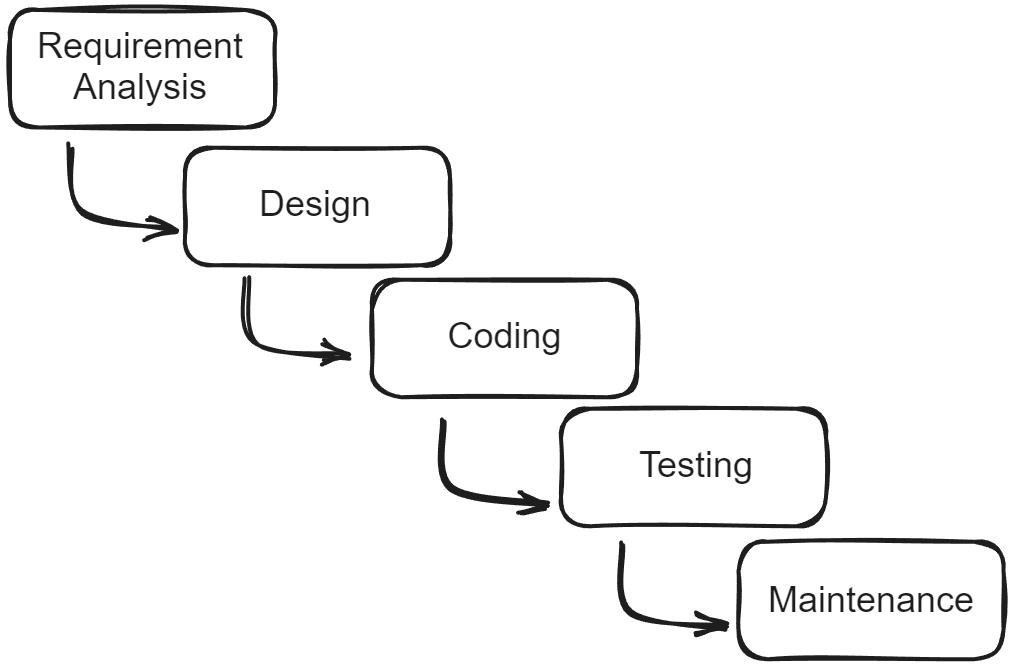
\includegraphics[width=0.65\textwidth]{texs/Part2/chapter1/image/waterfall.png}
	\caption{Waterfall Model}
	\label{fig:waterfall-model}
\end{figure}


\section{Model-View-Controller}
\label{sec:model-view-controller}

The Model-View-Controller (MVC) architecture is a design pattern commonly used in software development to separate the concerns of an application into three distinct components: the model, the view, and the controller \cite[47]{Garca2023}. The model represents the data and business logic of the application, the view is responsible for presenting the data to the user, and the controller handles user input and updates the model and view accordingly \cite{sarker14}.

The MVC architecture offers several benefits for software development. Firstly, it promotes code reusability by separating the different aspects of the application \cite{sarker14}. Additionally, MVC allows for multiple representations of the same information, enabling the creation of different views for different user interfaces \cite{sarker14}. This flexibility is particularly useful in interactive applications where users may have different preferences or requirements.

Another major advantage of MVC is that it allows for seperation of concerns \cite{Stepien}. By isolating the data, business logic, and presentation layers, developers can more easily understand and modify each component without affecting the others. This modularity improves the maintainability and scalability of the application, as changes can be made to one component without impacting the entire system \cite{Kozon_2023}.

Figure \ref{fig:mvc} shows the MVC architecture that will be utilized for this project.

\begin{figure}[!ht]
	\centering
	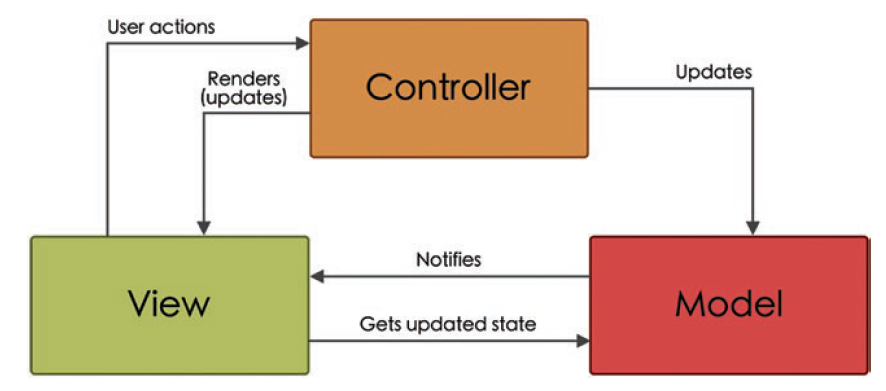
\includegraphics[width=0.65\textwidth]{texs/Part2/chapter1/image/mvc.png}
	\caption{Model-View-Controller Architecture \cite[46]{Garca2023}}
	\label{fig:mvc}
\end{figure}

\section{Thread Pool}
\label{sec:thread-pool}

A thread pool is a collection of worker threads that efficiently execute asynchronous callbacks on behalf of the application \cite{Karl-Bridge-Microsoft}. It is primarily used to reduce the number of application threads and provide management of the worker threads \cite{Karl-Bridge-Microsoft}.

The working principles of thread pool is relatively simple. It begins by initializing a pool of threads, or sometimes referred to as worker or executor. The number of threads in the pool is usually dependent on the number of cores in the CPU \cite{GeekforGeek_2020}. Too large thread pool size can results in resource trashing, where time is wasted in context switching between threads \cite{GeekforGeek_2020}.

When threads creation is completed, they are now ready for execution , while task can now be created and placed inside a queue \cite{GeekforGeek_2020}. Threads that are idle will then be assigned to the task in the queue and once the task is completed, the thread will be returned to the pool for reuse \cite{GeekforGeek_2020}. If all threads are busy, the task will be placed in the queue and wait for an available thread to be assigned to it \cite{GeekforGeek_2020}.

Figure \ref{fig:thread-pool} shows an overview on thread pool architecture.

\begin{figure}[!ht]
	\centering
	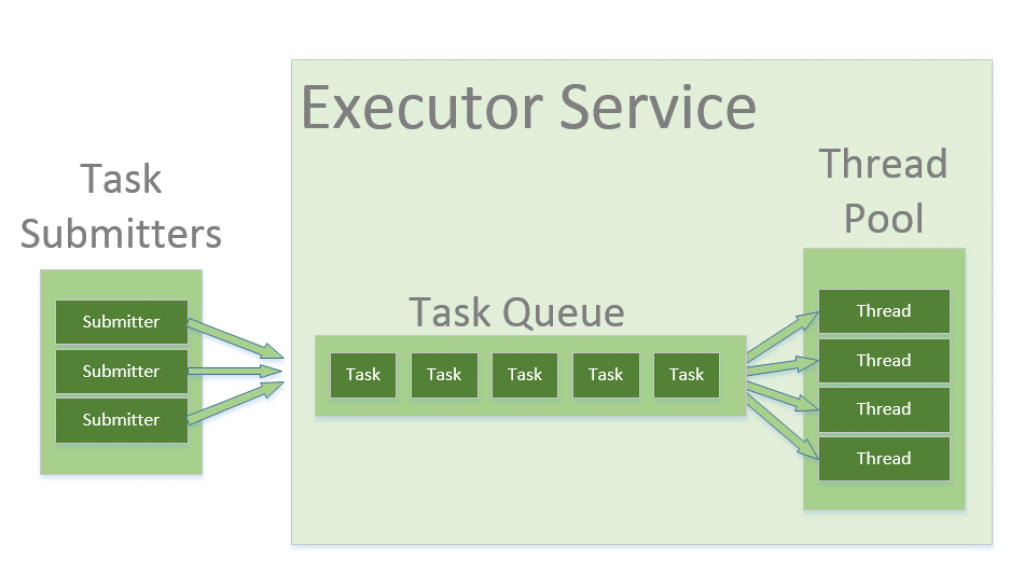
\includegraphics[width=0.65\textwidth]{texs/Part2/chapter1/image/threadpool.png}
	\caption{Thread Pool Architecture \cite{Paraschiv_2023}}
	\label{fig:thread-pool}
\end{figure}